% \begin{itemize}
%     \item What is a porous material? 
%     \begin{itemize}
%         \item What makes them different to non-porous materials?
%         \item Why do their differences make them industrially relevant?
%         \item What are some synthesis techniques that exist?
%         \item What are weaknesses with those synthesis techniques?
%     \end{itemize}
%     \item What is a particle stabilized emulsion
%     \begin{itemize}
%         \item Why are they interesting for porous material applications?
%         \item What is a bijel?
%         \item How are bijels relevant to porous materials?
%         \item Fabrication techniques that are proposed which allow large scale bijel fabrication
%         \item microstructure control in those applications
%     \end{itemize}
%     \item Purpose of study
%     \begin{itemize}
%         \item Three aims of the study 
%         \item significance of study
%         \item assumptions and limitations of the study
%     \end{itemize}
%     \item Summary of motivation, purpose and research aims
% \end{itemize}

% \textcolor{blue}{
% \begin{itemize}
%   \item Explain what is a porous material and the advantages they have in their applications compared to non-porous materials 
%   \item Detailed description of their applications and why we are interested in stimuli responsive porous materials 
%   \item Overview of porous material synthesis techniques and what are some areas where there is room for improvement (Definition of critical issues)
%   \item Explain what emulsion templating is and the specific advantages it has over other techniques. Recall where it has been used to great effect
%   \item Explain how bijels fit into emulsion templating and how they offer advantages to standard emulsion templates
%   \item Explain how bijels have been manufactured
%   \item Linking stimuli response as a way to add additional functionality to bijels and identifying how to process them more effectively
%   \item Explain why magnetic fields are interesting in this case
%   \item Explain what is a bijel, how they have been synthesized and some hints at past work for controlling their microstructure (literature review)
%   \item Explain how bijels and stimuli response can address the shortcomings addressed in the previous section (Research objectives)
% \end{itemize}
% }

\section{Introduction}
\label{section:introduction}

Porous materials play a vital role across a range of applications, including water filtration, catalyst supports, battery electrodes, and bioengineered 
materials. These materials are characterized by a network of pores that significantly increase surface area-to-volume ratio compared to their 
homogeneous counterparts. According to the IUPAC classification, porous materials are defined by their pore sizes as microporous ($L < 2$ nm), 
mesoporous ($2 < L < 50$ nm), or macroporous ($L > 50$ nm) \cite{sing_reporting_1985}. Experimental techniques such as BET analysis have shown 
that porous materials can possess surface areas exceeding those of solid materials by orders of magnitude \cite{shimizu_surface_2022}. The internal 
structure, including pore distribution and connectivity, also influences material performance and is often quantified by tortuosity 
\cite{chen_tortuosity_2020, ebner_tortuosity_2014}.

To meet increasing demands for tunable porosity, bottom-up synthesis strategies have gained traction. Among them, emulsion templating has emerged as a 
versatile technique that leverages phase separation to produce complex porous architectures. One particularly promising class of emulsion-templated 
materials is bicontinuous interfacially jammed emulsion gels (bijels), which form through the arrested spinodal decomposition of partially miscible 
fluids. Stabilized by colloidal particles that adsorb onto the fluid interface, bijels exhibit a tortuous, co-continuous structure well-suited for 
applications requiring high surface area and tunable transport properties \cite{stratford_colloidal_2005, herzig_bicontinuous_2007, lee_bicontinuous_2010}. 
Their bottom-up formation approach enables scalable synthesis of porous templates for a variety of material systems such as battery electrodes, shown in
Figure \ref{fig:bijel_template} 
\cite{cha_bicontinuous_2019, samdani_bicontinuous_2017, thorson_bijel-templated_2019}.

\begin{figure}
    \centering
    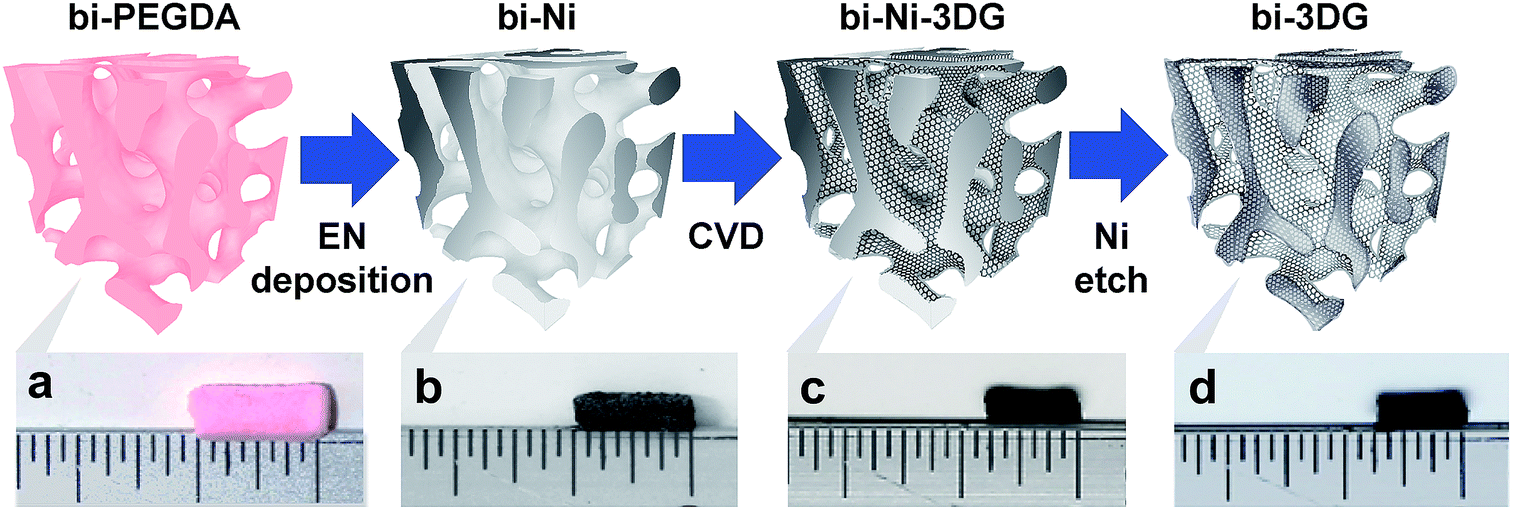
\includegraphics[scale = 0.5]{figures/introduction/bijel_templating.png}
    \caption{Fabrication of a graphite oxide battery electrode using bijel template. Used with permission of 
    Royal Society of Chemistry, from Scalable synthesis of gyroid-inspired freestanding three-dimensional graphene architectures, 
    Garcia et al., 1, 10, 2018 permission conveyed through Copyright Clearance Center, Inc}
    \label{fig:bijel_template}
\end{figure}

Fabrication methods for bijels have evolved from thermally induced spinodal decomposition (TIPS) to include solvent transfer-induced phase separation (STrIPS), 
vapor-induced phase separation (VIPS), and other advanced techniques \cite{haase_continuous_2015, wang_scalable_2020, amirfattahi_fabrication_2024}. 
These approaches allow for continuous production and offer access to various material shapes such as fibers, membranes, and capsules 
\cite{boakye-ansah_controlling_2020, kharal_hightensile_2020}. However, a key limitation is that the microstructure of bijels remains 
strongly tied to the casting mixture composition and phase separation kinetics. Adjusting the microstructure typically requires tuning 
component concentrations or altering flow conditions, which may be impractical or undesired in certain applications 
\cite{haase_continuous_2015, reeves_particle-size_2015}. 

% microstructure modification post synthesis
Once fabricated, the microstructure of bijels cannot be changed. In many applications proposed for bijels such as water filtration membranes
or drug release platforms, the microstructure of the material controls the back pressure, selectivity for specific species and transport
dynamics in the material. \cite{vanoli_bijels_2022, thorson_bijel-templated_2019} Creating a material whose microstructure an be dynamically
adjusted to the desired output parameters would add additional functionality and use cases for bijels. 

\begin{figure}[h]
    \centering
    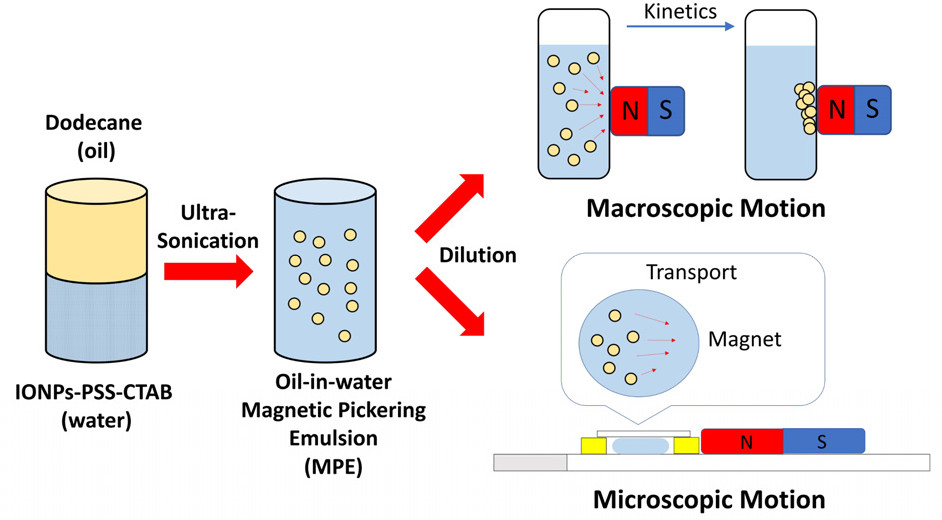
\includegraphics[scale = 1.5]{figures/introduction/magnetophoresis_emulsion.jpeg}
    \caption{Enhanced oil recovery of oil from water using magnetically responsive emulsion stabilizers, allowing for 
             locomotion and controlled coalescence of cargo from a matrix phase using magnetic fields. \cite{tham_magnetophoresis_2021} 
             K. Tham, W. M. Ng, S. S. Leong, S. P. Yeap, S. C. Low, H. L. Lee and J. Lim. Magnetophoresis of magnetic pickering 
             emulsions under low field gradient: Macroscopic and microscopic motion. 37, 1811: Reprinted (adapted) with permission from 
             Langmuir 2021, 37, 5, 1811-1822. Copyright 2025 American Chemical Society.}
    \label{fig:magnetophoresis_droplet}
\end{figure}

Stimuli-responsive strategies offer an attractive alternative for post-synthetic or in-situ control of bijel microstructures. External fields, 
pH, and temperature have all been explored to modify emulsion morphologies, particularly in Pickering emulsions 
\cite{tham_magnetophoresis_2021, cui_stabilizing_2013}. In Pickering emulsions, magnetically responsive particles have enabled droplet
manipulation, deformation, and coalescence control, shown in Figure \ref{fig:magnetophoresis_droplet}. By contrast, similar stimuli-responsive 
behaviors in bijels remain underexplored. Prior work with spherical particles under magnetic fields has shown limited microstructural modification 
\cite{kim_bijels_2010}, while electric fields have demonstrated greater influence \cite{carmack_tuning_2018}.

\begin{figure}[h]
    \centering
    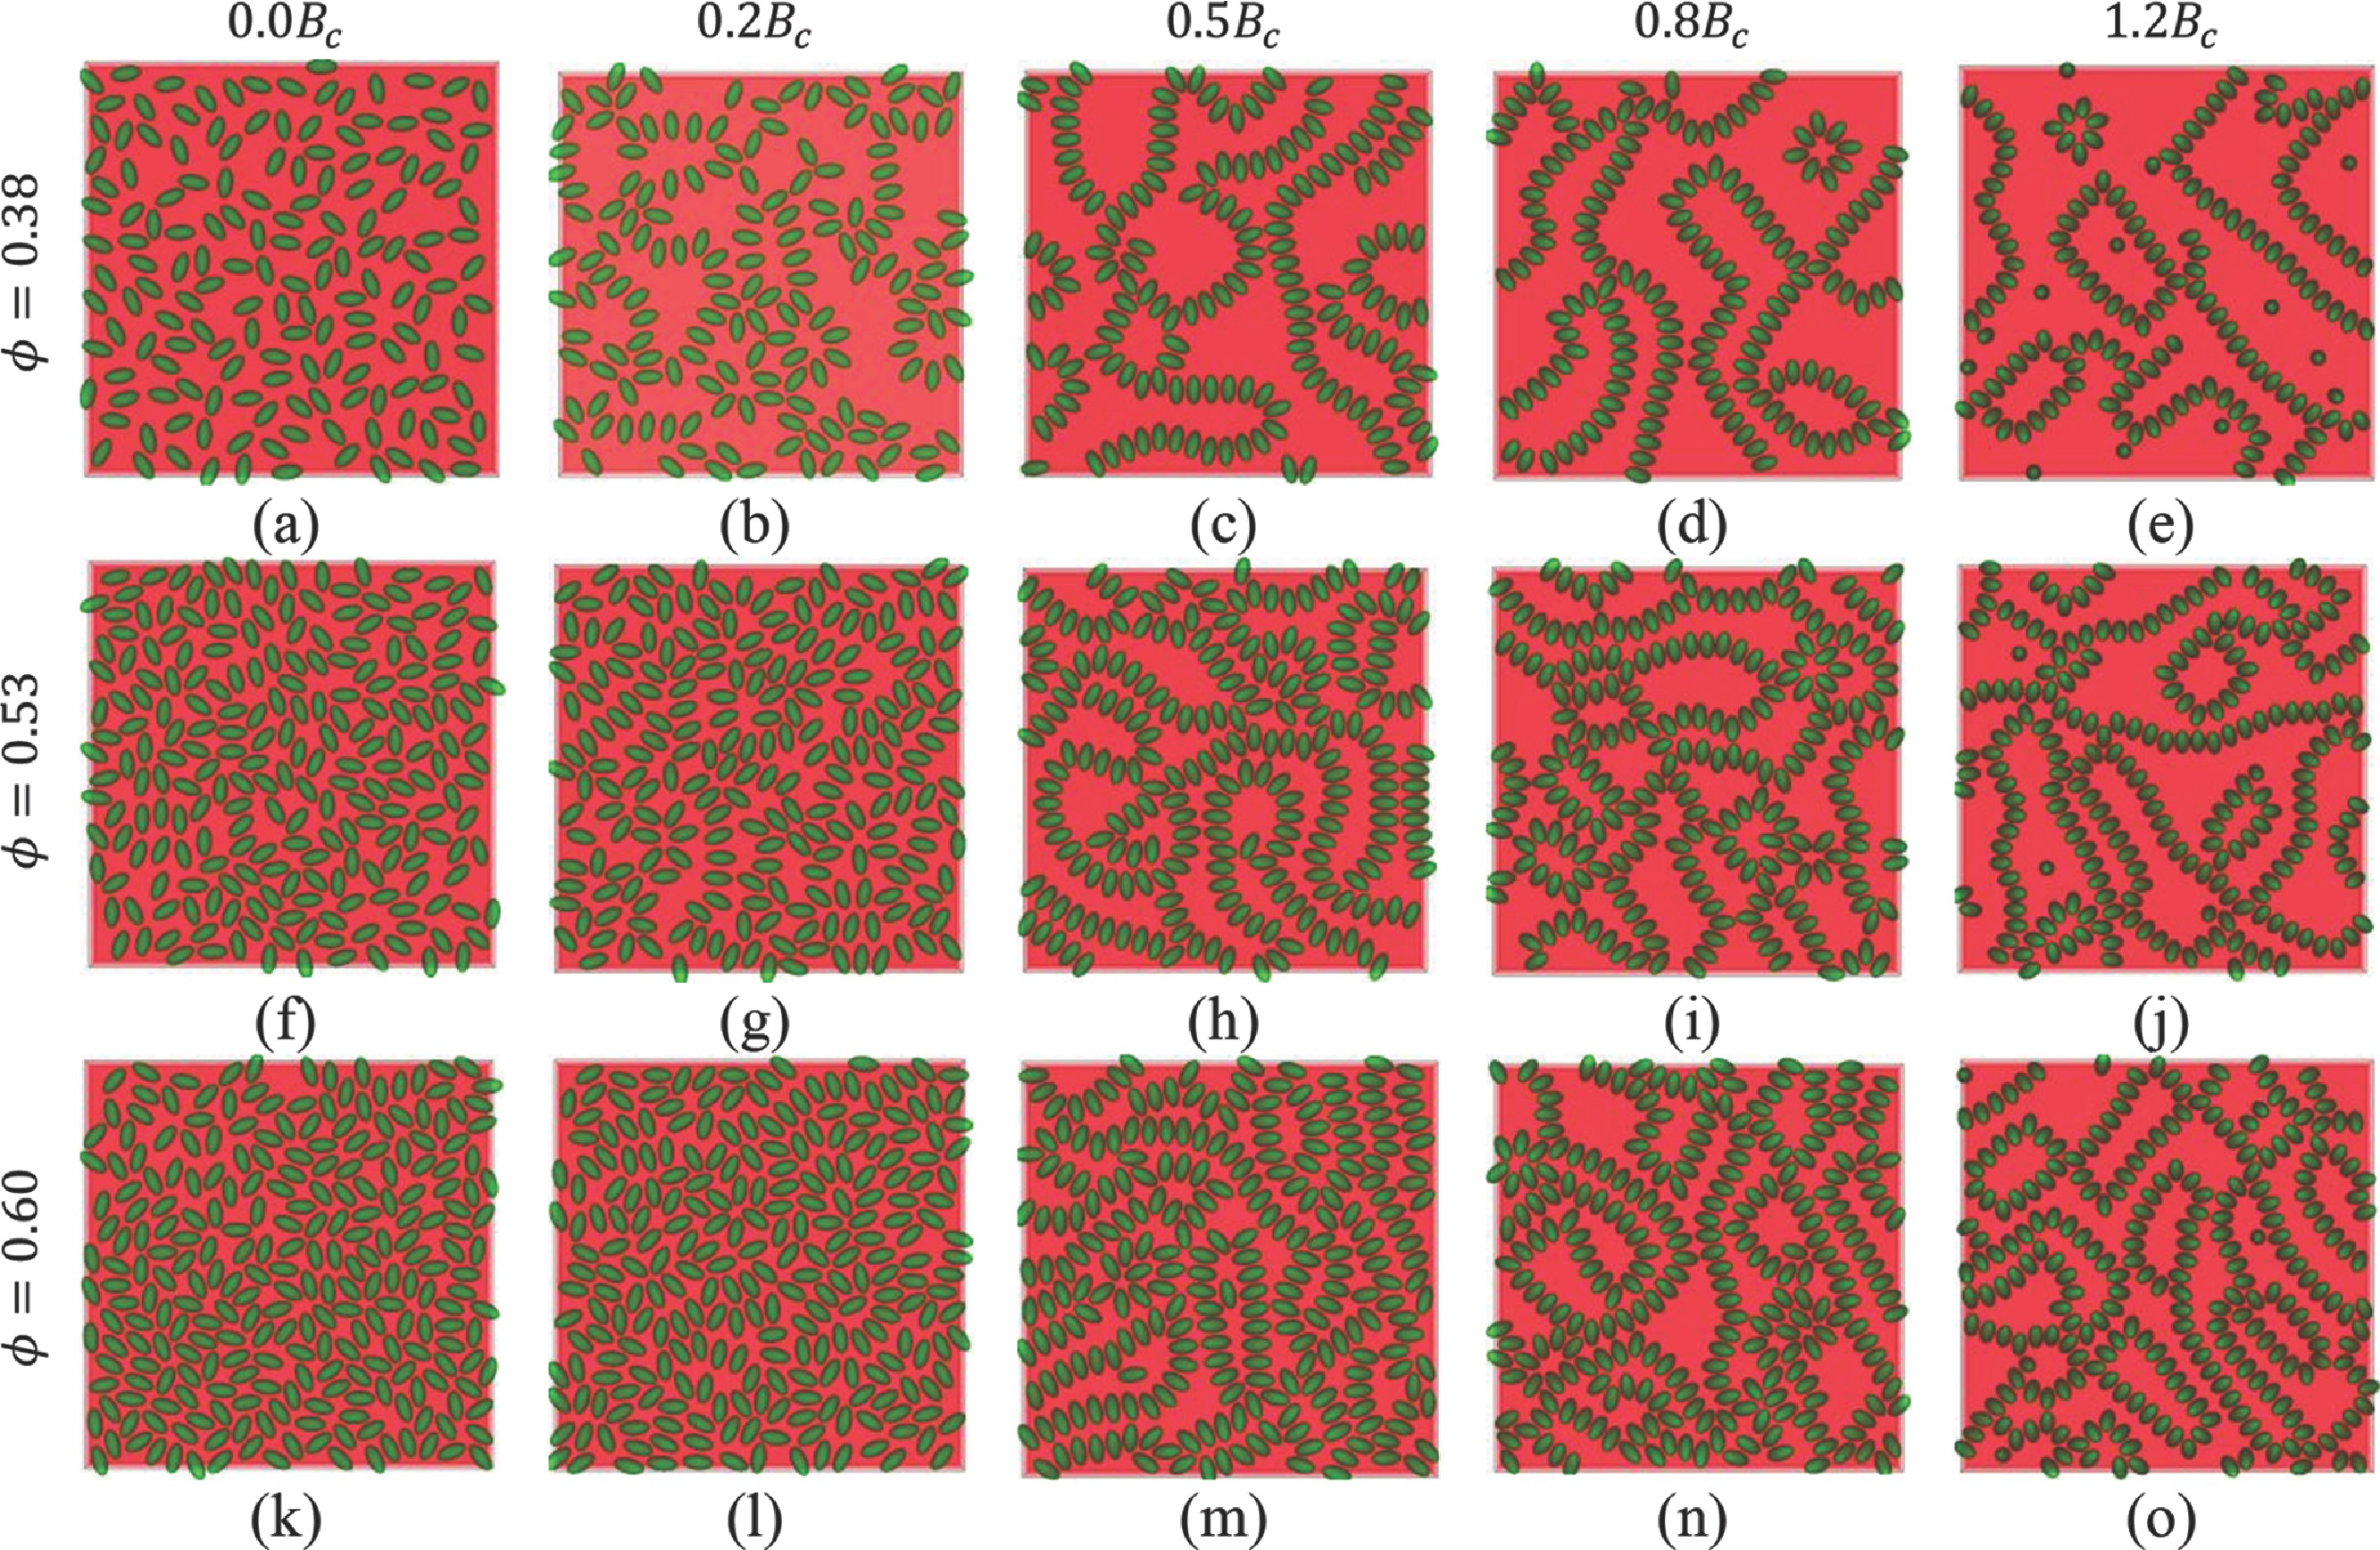
\includegraphics[scale = 0.4]{figures/introduction/anisotropic_particles_assembly.jpg}
    \caption{Assembly of prolate particles on a flat interface at various interfacial coverages and field strengths,
             showing the self assembly into chains that ellipsoidal particles can undergo under applied magnetic fields at
             interfaces. \cite{davies_assembling_2014} Reproduced from Davies et al. Adv. Mater., 26: 6715-6719 under the 
             Creative Commons CC BY license.}
    \label{fig:anisotropic_assembly}
\end{figure}

Recent advances suggest that anisotropic particles, particularly ellipsoidal particles, may offer enhanced responsiveness due to their shape-dependent 
interfacial behavior. When subjected to magnetic fields, ellipsoidal particles can align directionally, inducing local anisotropy in the interfacial 
packing arising from capillary deformation of the interface. This property has been characterized to induce self assembly of particles, 
shown in Figure \ref{fig:anisotropic_particle_interface} 
\cite{bresme_orientational_2007, davies_assembling_2014, newton_influence_2014}. By utilizing the magnetic field driven re-orientation and self assembly 
of particles at interfaces, the microstructure of bijels could be influenced pre and post formation. Therefore, leveraging this behavior offers a 
pathway to decouple microstructure control from casting mixture composition, expanding the design space for bijel derived porous materials and
soft matter.

The rheological properties are also of interest in bijels, owing to their synthesis and applications being tied to their rheology. STrIPS relied upon the
flow of casting mixture into a solvent bath and the rheological properties of the bijel are needed to ascertain the parameters to operate. 
\cite{haase_situ_2016, haase_continuous_2015} Additionally,
the uses of bijels in many applications such as cross-flow reactors are limited by the yielding of the particle monolayer under strain and fluid 
composition induced shear. \cite{boakye-ansah_controlling_2020} Magnetically responsive fluids have been shown to have significant increases in viscosity
due to particle ordering to the field increasing the fluids viscosity. When investigating the failure mechanism of bijels stabilized by spherical
particles under shear, previous investigations have shown that the particles align to the direction of shear before being pulled out of the interface.
\cite{bonaccorso_shear_2020} Therefore, magnetic fields affecting the orientation of particles at interfaces would be used to modify the rheological 
properties of bijels.

This dissertation investigates the potential of magnetically responsive ellipsoidal particles to enable stimuli-responsive control of bijel microstructure. 
Specifically, it explores whether magnetic fields applied during or after formation can induce meaningful microstructural changes, and how these changes 
influence the rheological properties of the resulting materials. The central hypothesis is that particle reorientation under magnetic fields alters 
interfacial packing, modifying the jamming threshold and thus the resulting domain morphology. By quantifying these effects across different processing 
conditions, this work aims to establish new methods for tunable bijel synthesis.

The remainder of this dissertation is structured as follows. Chapter 2 provides a review of the literature on the microstructures and factors affecting
particle stabilized emulsion and bijel formation, synthesis techniques for bijels and rheology of bijels. Chapter 3 outlines the simulation methods 
employed, including the Lattice Boltzmann approach and magnetic dipole modeling. Chapter 4 examines the impact of magnetic fields applied during bijel 
formation, characterizing changes in domain structure and particle ordering. Chapter 5 explores post-formation responsiveness by analyzing unjamming 
and reordering effects. Chapter 6 evaluates the rheological consequences of microstructural modifications, focusing on yield stress and shear-thinning 
behavior. Finally, Chapter 7 summarizes the findings and discusses their implications for the design of tunable porous materials, as well as some 
future avenues of exploration uncovered during this investigation.